\documentclass[12pt,twoside,openany]{book}

% Apply template settings. Unless you want to edit the template
% to match your needs, you don't want to mess with this file.
% Reference style
\usepackage[
    backend=biber,
	citestyle=ieee,
    maxbibnames=6,
    minbibnames=1,
    giveninits=true,
]{biblatex}
    
% Specify the margins.
\usepackage[a4paper, top=30mm, left=36mm, right=18mm, bottom=30mm, headheight=1mm, headsep=15mm, asymmetric]{geometry}

%\usepackage{eso-pic}					% Packages for layout and graphics 
\usepackage{graphicx}
\usepackage{tikz}
\usepackage{tocloft}                    % customize table of contents
\usepackage{etoc} 						% Separate tocs for appendix and the rest
\usepackage[titletoc,title]{appendix}
\usepackage{wrapfig}                    % Wrap text around figures
\usepackage{booktabs}					% Table formatting
\usepackage{titlesec}                   % Customize headers
\usepackage{fancyhdr}					% Setting the style for header and footer.
\usepackage{tabularx}
\usepackage{multirow}                   % For better tables 
\usepackage[hidelinks]{hyperref}		% Clickable links
\usepackage{nameref}					% References with names
\usepackage{ragged2e}                   % Better text alignment
\usepackage{lipsum}                     % Lipsum text

\usepackage{amsmath}

\usepackage{caption}                % customize caption labels and text
\usepackage{fontspec}               % select font by name
\usepackage{sectsty}                % customize font size, family, and style of section headings
\usepackage{csquotes}               % needed by babel/polyglossia

% Use 1.5 row spacing
\usepackage{setspace}
\onehalfspacing

% Set space between items in lists
\usepackage{enumitem}
\setlist[itemize]{itemsep=0pt,leftmargin=*}
\setlist[enumerate]{itemsep=0pt,leftmargin=*}

% Specify fonts
\setmainfont{Georgia}
\setsansfont{Arial}
\newfontfamily\footerfont{Georgia}

% Avoid hyphenation
% Try to lower the values if you get lines with 4-5 words and wide spaces inbetween
\hyphenpenalty=10000
\tolerance=2500

\chapterfont{\RaggedRight\sffamily\Large}
\sectionfont{\RaggedRight\sffamily\large}
\subsectionfont{\RaggedRight\sffamily\normalsize}
\subsubsectionfont{\RaggedRight\sffamily\normalsize}
\renewcommand{\familydefault}{\rmdefault}

% Style Contents
\renewcommand*\cfttoctitlefont{\Large\bf\sffamily}      % Title
\renewcommand\cftchapfont{\large\bf\sffamily}           % Chapter
\renewcommand\cftchappagefont{\large\bf\sffamily}       % Chapter page
\renewcommand\cftsecfont{\normalsize\bf\sffamily}       % Section
\renewcommand\cftsecpagefont{\normalsize\bf\sffamily}   % Section page
\renewcommand\cftsubsecfont{\normalsize\sffamily}       % Subsection
\renewcommand\cftsubsecpagefont{\normalsize\sffamily}   % Subsection page

% Style List of Figures
\renewcommand*\cftloftitlefont{\Large\bf\sffamily}      % Title
\renewcommand\cftfigfont{\normalsize\sffamily}          % Entry
\renewcommand\cftfigpagefont{\normalsize\sffamily}      % Entry page

% Style List of Tables
\renewcommand*\cftlottitlefont{\Large\bf\sffamily}      % Title
\renewcommand\cfttabfont{\normalsize\sffamily}          % Entry
\renewcommand\cfttabpagefont{\normalsize\sffamily}      % Entry page

% Define table column type for centered paragraph
\newcolumntype{C}[1]{>{\centering\arraybackslash}p{#1}}

% Format captions in wrapped figures
\newfontfamily\arialcaptionfont{Arial}[SizeFeatures={Size=10}]
\DeclareCaptionFont{caption}{\arialcaptionfont}
\captionsetup{
    font=caption,
    format=hang,
    singlelinecheck=off,
    justification=justified,
}

% Style the header and footer
\fancyhf{}
\fancyhead[LE]{\scriptsize\sffamily \thepage \quad|\quad \MakeUppercase\leftmark} % LE: Left side of Even pages
% Configuration for odd (right) pages: "Chapter Title | pageNumber"
\fancyhead[RO]{\scriptsize\sffamily \MakeUppercase\leftmark \quad|\quad \thepage} % RO: Right side of Odd pages
% Optional: Customize the appearance of chapter titles in the header
\renewcommand{\chaptermark}[1]{%
  \markboth{#1}{}%
}
\renewcommand{\headrulewidth}{0pt}

% Adjust chapter heading formatting to include chapter number
\titleformat{\chapter}[block] % 'block' style for the title
  {\sffamily\Large\bfseries} % Font styling
  {\thechapter\ } % Label for the chapter number
  {25pt} % Separation between label and title
  {} % Before the title code
  
% Add extra margin before the title of a new chapter
\titlespacing*{\chapter}
  {0pt} % Left margin
  {20mm} % Top margin
  {20pt} % Bottom margin


\fancypagestyle{plain}{
    \fancyhf{}
    % Add left-adjusted header text "pageNumber | CHAPTER TITLE" to even pages
    % LE: Left side of Even pages
    \fancyhead[LE]{\scriptsize\sffamily \thepage \quad|\quad \MakeUppercase\leftmark}
    
    % Add right-adjusted header text "CHAPTER TITLE | pageNumber" to odd pages
    % RO: Right side of Odd pages
    \fancyhead[RO]{\scriptsize\sffamily \MakeUppercase\leftmark \quad|\quad \thepage}
    
    % Optional: Customize the appearance of chapter titles in the header
    \renewcommand{\chaptermark}[1]{%
      \markboth{##1}{}%
    }
    \renewcommand{\headrulewidth}{0pt}
}

\fancypagestyle{none}{
  \fancyhf{}
  \renewcommand{\headrulewidth}{0pt}
  \renewcommand{\footrulewidth}{0pt}
}

\pagestyle{fancy}

% Languages
\usepackage[english,swedish]{babel} % The last is default
\usepackage{iflang}

% Define bibliography file
\addbibresource{references.bib}

% Make Swedish titles comply with instructions
\addto\captionsswedish{
    \renewcommand{\contentsname}{Innehållsförteckning}
    \renewcommand{\listfigurename}{Figurförteckning}
    \renewcommand{\listtablename}{Tabellförteckning}
}

% Custom unnumbered chapter that ensures the chapter title in the header is updated
\newcommand{\unnumberedchapter}[1]{
    \chapter*{#1}
    \markboth{#1}{#1}
}

\begin{document}
\raggedbottom

% Change this to reflect your thesis language
% Valid values: english or swedish
\selectlanguage{english}

% Remove or comment out this line to get rid of the README
\newgeometry{
    top=20mm,
    left=25mm,
    right=40mm,
    bottom=20mm
}
    
\section*{README}
\thispagestyle{empty}

\newcommand{\email}[1]{\href{mailto:#1}{\nolinkurl{#1}}}

{%
    \fontsize{12pt}{15pt}\selectfont
    This template is designed for master's theses at the INDEK department of KTH Royal Institute of Technology. It was created in January 2024 by Viktor Mörsell\footnote{<\email{viktor@upper.st}; \email{morsell@kth.se}>.}, based on the excellent ICT thesis template by Hannes Rabo\footnote{<\email{hannes.rabo@gmail.com}; \email{hrabo@kth.se}>.}. If you encounter any issues, please feel free to reach out. The template is made available on GitHub\footnote{\url{https://github.com/vmorsell/indek-master-thesis-template-latex}} "as is" and strives to adhere to:
    
    \begin{itemize}
        \item INDEK Thesis Instructions v6\footnote{\url{https://www.kth.se/polopoly_fs/1.1172225.1662124048!/X-jobbsrapport\%20-\%20INSTRUKTION\%20f\%C3\%A4rdigst\%C3\%A4llande\%20v6.pdf}}
        \item INDEK First Pages Example v4\footnote{\url{https://www.kth.se/polopoly_fs/1.1172231.1662124088!/X-jobbsrapport\%20CINEK\%20-\%20EXEMPEL\%20F\%C3\%B6rsta\%20sidorna\%20v4.pdf}}
        \item Selected aspects of KTH's General Rules for Covers and Inlays\footnote{\url{https://www.kth.se/polopoly_fs/1.487233.1584470685!/Tips_utformning_avhandling.pdf}}
        \item The IEEE Journals Reference Format\footnote{\url{http://journals.ieeeauthorcenter.ieee.org/wp-content/uploads/sites/7/IEEE_Reference_Guide.pdf}}
    \end{itemize}

    \noindent The sample content provided aims to demonstrate formatting styles and layout options. Ensure you customize the structure to suit your research needs and follow your supervisor's guidelines.

    \subsection*{Getting started}

    \begin{enumerate}
        \item Choose the language for your thesis in \texttt{main.tex}
        \item Modify the thesis structure in \texttt{main.tex} as required
        \item Update the files in the \texttt{content/} directory
        \item Add or delete chapters according to your thesis needs
        \item To remove this README, comment out the line below in \texttt{main.tex}
        \vspace*{-1.1em}\begin{verbatim}
\newgeometry{
    top=20mm,
    left=25mm,
    right=40mm,
    bottom=20mm
}
    
\section*{README}
\thispagestyle{empty}

\newcommand{\email}[1]{\href{mailto:#1}{\nolinkurl{#1}}}

{%
    \fontsize{12pt}{15pt}\selectfont
    This template is designed for master's theses at the INDEK department of KTH Royal Institute of Technology. It was created in January 2024 by Viktor Mörsell\footnote{<\email{viktor@upper.st}; \email{morsell@kth.se}>.}, based on the excellent ICT thesis template by Hannes Rabo\footnote{<\email{hannes.rabo@gmail.com}; \email{hrabo@kth.se}>.}. If you encounter any issues, please feel free to reach out. The template is made available on GitHub\footnote{\url{https://github.com/vmorsell/indek-master-thesis-template-latex}} "as is" and strives to adhere to:
    
    \begin{itemize}
        \item INDEK Thesis Instructions v6\footnote{\url{https://www.kth.se/polopoly_fs/1.1172225.1662124048!/X-jobbsrapport\%20-\%20INSTRUKTION\%20f\%C3\%A4rdigst\%C3\%A4llande\%20v6.pdf}}
        \item INDEK First Pages Example v4\footnote{\url{https://www.kth.se/polopoly_fs/1.1172231.1662124088!/X-jobbsrapport\%20CINEK\%20-\%20EXEMPEL\%20F\%C3\%B6rsta\%20sidorna\%20v4.pdf}}
        \item Selected aspects of KTH's General Rules for Covers and Inlays\footnote{\url{https://www.kth.se/polopoly_fs/1.487233.1584470685!/Tips_utformning_avhandling.pdf}}
        \item The IEEE Journals Reference Format\footnote{\url{http://journals.ieeeauthorcenter.ieee.org/wp-content/uploads/sites/7/IEEE_Reference_Guide.pdf}}
    \end{itemize}

    \noindent The sample content provided aims to demonstrate formatting styles and layout options. Ensure you customize the structure to suit your research needs and follow your supervisor's guidelines.

    \subsection*{Getting started}

    \begin{enumerate}
        \item Choose the language for your thesis in \texttt{main.tex}
        \item Modify the thesis structure in \texttt{main.tex} as required
        \item Update the files in the \texttt{content/} directory
        \item Add or delete chapters according to your thesis needs
        \item To remove this README, comment out the line below in \texttt{main.tex}
        \vspace*{-1.1em}\begin{verbatim}
\newgeometry{
    top=20mm,
    left=25mm,
    right=40mm,
    bottom=20mm
}
    
\section*{README}
\thispagestyle{empty}

\newcommand{\email}[1]{\href{mailto:#1}{\nolinkurl{#1}}}

{%
    \fontsize{12pt}{15pt}\selectfont
    This template is designed for master's theses at the INDEK department of KTH Royal Institute of Technology. It was created in January 2024 by Viktor Mörsell\footnote{<\email{viktor@upper.st}; \email{morsell@kth.se}>.}, based on the excellent ICT thesis template by Hannes Rabo\footnote{<\email{hannes.rabo@gmail.com}; \email{hrabo@kth.se}>.}. If you encounter any issues, please feel free to reach out. The template is made available on GitHub\footnote{\url{https://github.com/vmorsell/indek-master-thesis-template-latex}} "as is" and strives to adhere to:
    
    \begin{itemize}
        \item INDEK Thesis Instructions v6\footnote{\url{https://www.kth.se/polopoly_fs/1.1172225.1662124048!/X-jobbsrapport\%20-\%20INSTRUKTION\%20f\%C3\%A4rdigst\%C3\%A4llande\%20v6.pdf}}
        \item INDEK First Pages Example v4\footnote{\url{https://www.kth.se/polopoly_fs/1.1172231.1662124088!/X-jobbsrapport\%20CINEK\%20-\%20EXEMPEL\%20F\%C3\%B6rsta\%20sidorna\%20v4.pdf}}
        \item Selected aspects of KTH's General Rules for Covers and Inlays\footnote{\url{https://www.kth.se/polopoly_fs/1.487233.1584470685!/Tips_utformning_avhandling.pdf}}
        \item The IEEE Journals Reference Format\footnote{\url{http://journals.ieeeauthorcenter.ieee.org/wp-content/uploads/sites/7/IEEE_Reference_Guide.pdf}}
    \end{itemize}

    \noindent The sample content provided aims to demonstrate formatting styles and layout options. Ensure you customize the structure to suit your research needs and follow your supervisor's guidelines.

    \subsection*{Getting started}

    \begin{enumerate}
        \item Choose the language for your thesis in \texttt{main.tex}
        \item Modify the thesis structure in \texttt{main.tex} as required
        \item Update the files in the \texttt{content/} directory
        \item Add or delete chapters according to your thesis needs
        \item To remove this README, comment out the line below in \texttt{main.tex}
        \vspace*{-1.1em}\begin{verbatim}
\include{template/readme}
        \end{verbatim}
    \end{enumerate}
    
    \noindent Wishing you the very best of luck.

    \vspace{.69em}

    \noindent Stay curious,\\
    \textit{Viktor}

    \newpage
    \thispagestyle{empty}
    \vspace*{8em}
    \begin{quote}
        \centering
        \textit{You look lovely today!}\\
    \end{quote}
}

\clearpage % End the content with custom margins
\restoregeometry % Revert to the original margins
        \end{verbatim}
    \end{enumerate}
    
    \noindent Wishing you the very best of luck.

    \vspace{.69em}

    \noindent Stay curious,\\
    \textit{Viktor}

    \newpage
    \thispagestyle{empty}
    \vspace*{8em}
    \begin{quote}
        \centering
        \textit{You look lovely today!}\\
    \end{quote}
}

\clearpage % End the content with custom margins
\restoregeometry % Revert to the original margins
        \end{verbatim}
    \end{enumerate}
    
    \noindent Wishing you the very best of luck.

    \vspace{.69em}

    \noindent Stay curious,\\
    \textit{Viktor}

    \newpage
    \thispagestyle{empty}
    \vspace*{8em}
    \begin{quote}
        \centering
        \textit{You look lovely today!}\\
    \end{quote}
}

\clearpage % End the content with custom margins
\restoregeometry % Revert to the original margins

% Enumerate the front matter with Roman numbers
\pagenumbering{roman}

% Add cover page, blank page, title pages, abstracts, dedication,
% acknowledgements, preface, contents, list of figures and
% list of tables.
% Comment out, or add pages, as per your preference
% Set up header and footer
\definecolor{coverpageblue}{HTML}{1954A6}
\fancypagestyle{coverpage}{
    \fancyhf{} % Clear the header/footer

    \newcommand{\coverpagelogosize}{26.5mm}%{31.611mm}
    \newcommand{\coverpagewordmarkwidth}{37.37mm}

    % Header with KTH logotype and wordmark
    \renewcommand{\headrulewidth}{0pt}
    \fancyheadoffset[L]{11.9mm}
    \fancyhead[L]{%
        \raisebox{\dimexpr \ht\strutbox-\height+4mm}{%
            
\includegraphics[width=26.5mm]{template/img/kth-logo.png}%
        }
    }
    \fancyheadoffset[R]{11.9mm}
    \fancyhead[R]{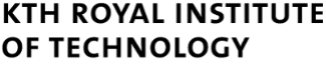
\includegraphics[width=37.37mm]{template/img/kth-name-text.png}}

    % Footer with blue line, city, country and year
    \renewcommand{\footrulewidth}{0pt}
    \fancyfoot[L]{%
        \vspace*{-13mm}
        \hspace*{-12mm}\color{coverpageblue}\rule{\dimexpr\paperwidth-27mm\relax}{1pt}%
    }
}

\newcommand{\makecoverfront}[8]{%
    {%
        \newpage
        \thispagestyle{coverpage}
        \newgeometry{
            top=11.6mm,
            left=25.3mm,
            right=25mm,
            bottom=13.8mm,
            headsep=43.5mm,
            includehead
        }
    
        \selectlanguage{#1}
        \sffamily
    
        {%
            \fontsize{12pt}{19pt}\selectfont
            \noindent\textit{#2}\par
            \noindent\textit{#3}\par
        }
    
        \vspace{36pt}
    
        {%
            \fontsize{26pt}{26pt}\selectfont
            \RaggedRight\textbf{#4}\par
        }
    
        \vspace{11pt}
    
        {%
            \fontsize{16pt}{16pt}\selectfont
            \RaggedRight#5\par
        }
    
        \vspace{1pt}
    
        {%
            \fontsize{12pt}{35pt}\selectfont
            \noindent\textbf{\MakeUppercase{#6}}\par
            \noindent\textbf{\MakeUppercase{#7}}\par
        }

        \vspace{\fill}

        {%
            \hspace*{-18mm}\sffamily\fontsize{8pt}{10pt}\selectfont%
            Stockholm, \iflanguage{english}{Sweden}{Sverige} #8
        }
        
        \clearpage
        \restoregeometry
    }
}

\makecoverfront
    {english}
    {Degree Project in Industrial Management}
    {Second cycle, 30 credits}
    {Ad minim veniam, quis nostrud exercitation ullamco laboris}
    {Nisi ut aliquip ex ea commodo consequat, duis aute irure dolor in reprehenderit}
    {Jane Smith}
    {John Doe}
    {2024}
\newpage
\thispagestyle{empty}
\mbox{}
\newcommand{\maketitlepage}[5]{%
    {%
        \newpage
        \pagestyle{empty}
        \newgeometry{
            left=20mm,
            top=80.5mm,
            right=20mm,
            bottom=30.5mm
        }
    
        {%
            \selectlanguage{#1}
            \sffamily
            
            {
                \centering
                {%
                    \fontsize{24pt}{24pt}\selectfont%
                    #2\par
                }

                {%
                    \fontsize{20pt}{20pt}\selectfont%
                    
                    \vspace{22pt}
                    \iflanguage{english}{by}{av}
                    \vspace{22pt}
                
                    #3 \\
                    \vspace{6pt}
                    #4
                    \par
                }
                
                \vspace*{\fill}
        
                {%
                    \fontsize{12pt}{13pt}\selectfont%
                    \iflanguage{english}{%
                        Master of Science Thesis TRITA-#5\\
                        KTH Industrial Engineering and Management\\
                        Industrial Economics and Management\\
                    }{%
                        Examensarbete TRITA-#5\\
                        KTH Industriell teknik och management\\
                        Industriell ekonomi och organisation\\
                    }
                    SE-100 44 STOCKHOLM\par
                }
            }
        }
        
        \clearpage
        \restoregeometry
    }
}

\maketitlepage
    {english}
    {Ad minim veniam, quis nostrud exercitation ullamco laboris}
    {Jane Smith}
    {John Doe}
    {ITM-EX 2024:XYZ}

\maketitlepage
    {swedish}
    {Svensk titel}
    {Jane Smith}
    {John Doe}
    {ITM-EX 2024:XYZ}
\newcommand{\makeabstractpage}[2]{
    {%
        \newpage
        \pagestyle{empty}
        \newgeometry{
            top=15mm,
            left=25mm,
            right=25mm,
            bottom=30mm
        }
        
        {%
            \selectlanguage{#1}
            
            #2
        }
        
        \clearpage
        \restoregeometry
    }
}

\newcommand{\makeabstractheader}[9]{
    {%
        \renewcommand{\familydefault}{\sffamily}
        \noindent\begin{tabular}{| p{0.22\textwidth} p{0.06\textwidth} p{0.3\textwidth} | p{0.36\textwidth} |}
        \hline
        \vspace*{-4pt}\multirow{5}{*}{%
            \vspace*{10pt}\iflanguage{english}{%
                
\includegraphics[width=31.611mm]{template/img/kth-itm-logo-en.jpg}
            }{%
                
\includegraphics[width=31.611mm]{template/img/kth-itm-logo-sv.jpg}
            }
            
        }
        &
        & \multicolumn{2}{C{0.68\textwidth}|}{%
            \sffamily\textbf{%
                \iflanguage{english}{Master of Science Thesis}{Examensarbete} TRITA-#1
            }
        }
        \\
        &
        &
        \multicolumn{2}{l|}{}
        \\
        &
        & \multicolumn{2}{C{0.68\textwidth}|}{%
            \sffamily\textbf{#2}
        }
        \\
        &
        & \multicolumn{2}{l|}{}
        \\
        &
        & \multicolumn{2}{C{0.68\textwidth}|}{\sffamily#3}
        \\
        &
        & \multicolumn{2}{C{0.68\textwidth}|}{\sffamily#4}
        \\
        \hline
        {%
            \sffamily\fontsize{7pt}{7pt}\selectfont%
            \iflanguage{english}{Approved}{Godkänd}
        }
        &
        \multicolumn{2}{|l|}{%
            \sffamily\fontsize{7pt}{7pt}\selectfont%
            \iflanguage{english}{Examiner}{Examinator}
        }
        &
        {%
            \sffamily\fontsize{7pt}{7pt}\selectfont%
            \iflanguage{english}{Supervisor}{Handledare}
        } \\
        \sffamily#5 &
        \multicolumn{2}{|p{0.33\textwidth}|}{\sffamily#6} &
        \sffamily#7 \\
            
        \hline
        &
        \multicolumn{2}{|l|}{%
            \sffamily\fontsize{7pt}{7pt}\selectfont%
            \iflanguage{english}{Commissioner}{Uppdragsgivare}
        } &
        {%
            \sffamily\fontsize{7pt}{7pt}\selectfont%
            \iflanguage{english}{Contact Person}{Kontaktperson}
        } \\
        &
        \multicolumn{2}{|p{0.33\textwidth}|}{\sffamily#8} &
        \sffamily#9 \\
        \hline
        \end{tabular}
    }
}

\makeabstractpage{english}{
    \makeabstractheader
        {ITM-EX 2024:XYZ}
        {Ad minim veniam, quis nostrud exercitation ullamco laboris}
        {Jane Smith}
        {John Doe}
        {2024-mm-dd}
        {Alex Johnson}
        {Maria Garcia}
        {Summit Group AB}
        {Emily Taylor}
    
    \section*{Abstract}
    
    \lipsum[2-3] % Sample text
    
    \vspace{\fill}
        
    \subsection*{Keywords}
    Exam, Master, Finally, Short-timer
}

\makeabstractpage{swedish}{
    \makeabstractheader
        {ITM-EX 2024:XYZ}
        {Svensk titel}
        {Jane Smith}
        {John Doe}
        {2024-mm-dd}
        {Alex Johnson}
        {Maria Garcia}
        {Summit Group AB}
        {Emily Taylor}
    
    \section*{Sammanfattning}
    
    \lipsum[4-5] % Sample text
    
    \vspace{\fill}
        
    \subsection*{Nyckelord}
    Examen, master, äntligen, ingapinnar
}
\newpage
\thispagestyle{empty}

\vspace*{14em}
    
{%      
    \centering
    \textit{In loving memory of}\\
    \textit{Rut Ingrid}
    \par
}
\unnumberedchapter{Acknowledgements}

\lipsum[8] % Example text
\newpage
\etocdepthtag.toc{mtchapter}
\etocsettagdepth{mtchapter}{subsection}
\etocsettagdepth{mtappendix}{none}
\thispagestyle{plain}
\tableofcontents

\listoffigures
\clearpage
\listoftables

\unnumberedchapter{Preface}


\lipsum[8-9] % placeholder text

\vspace{2em}

\noindent Stockholm, January 2024 \\
\noindent \textit{Jane and John}

% Enumerate the body with Arabic numbers
\cleardoublepage

% Start on a right side page to not mess up the alternate left/right
% header alignment pattern
\pagenumbering{arabic}

% Now it's time to include the actual content of the thesis
% List all the files from content/ you want to include
\chapter{Introduction}

\label{ch:introduction}

This document is designed primarily for visualization purposes, serving as a guide to showcase formatting and structuring. 

Chapter \ref{ch:introduction}, titled "\nameref{ch:introduction}", features one image  and one table. These examples are included to enrich the "List of Figures" and "List of Tables" sections, demonstrating how to effectively incorporate and reference such elements within a document. 

The subsequent chapters contain placeholder text. This example text is intended to illustrate potential content layouts and to further demonstrate text formatting options in a comprehensive manner.

In order to make the reference section visible, we also need some references \cite{liu2017} to display there\cite{jones2017,liu2017}.

\section{Background}

\begin{wrapfigure}{r}{0.5\textwidth}
    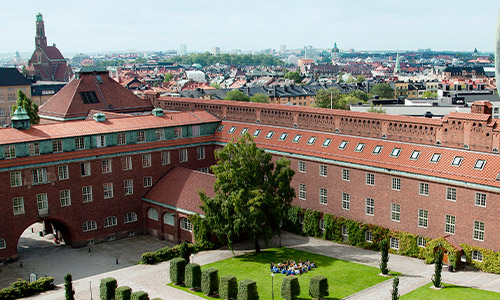
\includegraphics[width=\linewidth]{images/kth-courtyard.jpg}
    \caption{The KTH courtyard is a pretty neat place.}
    \label{fig:kth-courtyard}
\end{wrapfigure}

\lipsum[2]

\section{Problem}

\lipsum[3]

\begin{table}[ht]
    \centering
    \begin{minipage}{\textwidth}
        {\sffamily\textbf{Annual Sales Report}} \\
        {\sffamily{Fiscal Year 2023}} \\
        
        \begin{tabularx}{\textwidth}{ 
            >{\raggedright\arraybackslash}X 
            >{\raggedleft\arraybackslash}X 
            >{\raggedleft\arraybackslash}X 
            >{\raggedleft\arraybackslash}X 
            >{\raggedleft\arraybackslash}X }
            \toprule
            Product & Q1 Sales (\$) & Q2 Sales (\$) & Q3 Sales (\$) & Q4 Sales (\$) \\
            \midrule
            Product A & 25,000 & 27,000 & 24,000 & 29,000 \\
            Product B & 20,000 & 22,500 & 19,000 & 20,000 \\
            \bottomrule
        \end{tabularx}
        
        \caption{Sales numbers for the fiscal year 2023. This description is pretty long and spans over multiple lines.}
        \label{tab:sales-2023}
    \end{minipage}
\end{table}

\noindent\lipsum[4]

\subsection{Purpose and Research Question}

\lipsum[5] % placeholder text
\chapter{Literature Review}

\section{Key Concepts and Theories}
\lipsum[9] % placeholder text

\subsection{Lean Manufacturing}
\lipsum[7] % placeholder text

\section{Related Work}
\lipsum[10] % placeholder text
\chapter{Method}

\section{Research Design}
\lipsum[30] % placeholder text

\section{Data Collection}
\lipsum[33] % placeholder text

\subsection{Interviews}
\lipsum[35] % placeholder text

\subsection{Observations}
\lipsum[36] % placeholder text

\section{Ethical Aspect}
\lipsum[41] % placeholder text
\chapter{Results and Analysis}

\section{Data Presentation}
\lipsum[41] % placeholder text

\section{Analysis and Interpretation of Results}
\lipsum[42] % placeholder text
\chapter{Discussion}

\lipsum[50-52] % placeholder text
\chapter{Conclusions}
\lipsum[60-61] % placeholder text


% Finish up
\newpage
\printbibliography[heading=bibintoc,title={\iflanguage{english}{References}{Referenser}}]
\newpage

\begin{appendices}

% Add your appendices below
\chapter{First Appendix}
\lipsum[44-45] % placeholder text

\chapter{Second Appendix}
\lipsum[55-59] % placeholder text

\end{appendices}
% Header and footer
\definecolor{coverpageblue}{HTML}{1954A6}
\fancypagestyle{backcoverpage}{
    \fancyhf{} % Clear header & footer
    
    % Footer with KTH's website url
    \renewcommand{\footrulewidth}{0pt}
    \fancyfoot[L]{%
        \vspace*{-2.5mm}%
        {%
            \hspace*{-11.6mm}\color{coverpageblue}\sffamily\fontsize{8pt}{10pt}\selectfont%
            www.kth.se
        }
        \hspace*{-12mm}\color{coverpageblue}\rule{\dimexpr\paperwidth-28mm\relax}{1pt}%
    }
}

\newcommand{\makebackcoverpage}[1]{%
    {%
        \newgeometry{
            left=28.5mm,
            bottom=24mm,
        }
        
        \thispagestyle{backcoverpage}
        \sffamily
        
        \vspace*{\fill}
        
        \noindent\hspace*{-11.6mm}\fontsize{10pt}{10pt}\selectfont%
        TRITA-#1
        
        \clearpage
        \restoregeometry
    }
}
\makebackcoverpage{ITM-EX 2024:XYZ}

\end{document}